\documentclass[tikz,border=10pt]{standalone}
\usepackage{tikz}
\usetikzlibrary{calc}

\begin{document}
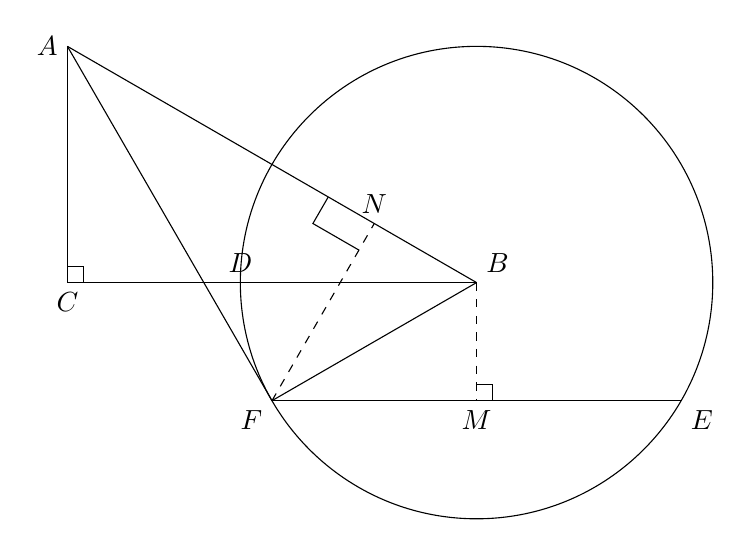
\begin{tikzpicture}
    % Define coordinates based on geometric analysis
    % B is the center (0,0)
    \coordinate (B) at (0,0);
    
    % C is to the left on the x-axis. Let's say distance 5.2 (approx 3*sqrt(3))
    \coordinate (C) at (-5.196, 0);
    
    % A is directly above C. Let's say height 3.
    \coordinate (A) at (-5.196, 3);
    
    % Circle centered at B with radius 3
    % D is the intersection of CB and the circle
    \coordinate (D) at (-3, 0);
    
    % F is on the circle. Based on tangency and perpendiculars, 
    % angle FBA is 60 degrees. A is at approx 150 deg. So F is at 210 deg.
    \coordinate (F) at (-2.598, -1.5);
    
    % E is on the circle, forming a horizontal chord FE with F
    \coordinate (E) at (2.598, -1.5);
    
    % M is the projection of B onto FE (midpoint of chord)
    \coordinate (M) at (0, -1.5);
    
    % N is the projection of F onto AB
    % Calculated as approx (-1.3, 0.75)
    \coordinate (N) at (-1.299, 0.75);

    % Draw the circle
    \draw (B) circle (3);

    % Draw solid lines
    \draw (A) -- (C);             % AC
    \draw (C) -- (B);             % CB (passes through D)
    \draw (A) -- (B);             % AB (passes through N)
    \draw (A) -- (F);             % AF
    \draw (F) -- (E);             % FE (passes through M)
    \draw (B) -- (F);             % Radius BF

    % Draw dashed lines
    \draw[dashed] (B) -- (M);     % BM
    \draw[dashed] (F) -- (N);     % FN

    % Draw right-angle marks
    % At C (AC perp CB)
    \draw (C) ++(0,0.2) -| ++(0.2,-0.2);
    
    % At M (BM perp FE) - mark in the angle BME
    \draw (M) ++(0,0.2) -| ++(0.2,-0.2);
    
    % At N (FN perp AB) - mark in the angle FNA
    \path (N) -- (A) coordinate[pos=0.15] (NA);
    \path (N) -- (F) coordinate[pos=0.15] (NF);
    \draw (NA) -- ($(NA) + (NF) - (N)$) -- (NF);

    % Labels
    \node[left] at (A) {$A$};
    \node[below] at (C) {$C$};
    \node[above] at (D) {$D$};
    \node[above right] at (B) {$B$};
    \node[above] at (N) {$N$};
    \node[below left] at (F) {$F$};
    \node[below] at (M) {$M$};
    \node[below right] at (E) {$E$};

\end{tikzpicture}
\end{document}
